\chapter{Literature review}
\label{chap:literaturereview}
	\textit{mentions some related studies on the use of machine techniques to detect malicious requests, their strengths and weaknesses and evaluate an appropriate approach for this thesis.}
	\minitoc

\section{U-Net}
\label{sec:u_net}
	U-Net do Ronneberger và cộng sự \cite{ronneberger2015u} đề xuất, là một mạng học sâu được phát triển cho công việc phân đoạn hình ảnh y khoa tại khoa Khoa học Máy tính của trường Đại học Freiburg, Đức. Kiến trúc của mạng này phù hợp để có thể huấn luyện với ít hình ảnh hơn nhưng lại thu được kết quả phân đoạn chính xác hơn. Quá trình phân đoạn cho một hình có kích thước 512$\times$512 diễn ra không quá một giây trên những GPU\nomenclature{GPU}{Graphics Processing Unit} đời mới. Nhờ đó, Ronneberger và cộng sự đã giành chiến thắng tại Thách thức theo dõi tế bào (Cell Tracking Challenge) ISBI\nomenclature{ISBI}{International Symposiom on Biomedical Imaging} 2015. Trong mục này, chúng tôi trình bày chi tiết về kiến trúc mạng và cách khởi tạo trọng số được sử dụng trong mạng U-Net.
	
\subsection{Kiến trúc mạng}
\label{subsec:kien_truc_mang_u_net}
	\begin{figure}[h!]
		\centering
		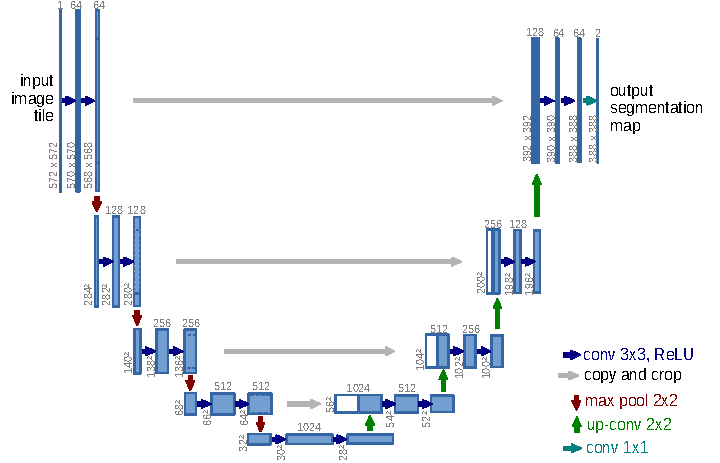
\includegraphics[width=0.9\linewidth]{figures/model_unet}
		\caption[Kiến trúc mô hình U-Net.]{Kiến trúc mô hình U-Net \sourcefig{\cite{ronneberger2015u}}.}
		\label{fig:kien_truc_mang_u_net}
	\end{figure}
	Kiến trúc mạng U-Net được mô tả trong \autoref{fig:kien_truc_mang_u_net}. Mô hình này bao gồm nhánh thu giảm ở bên trái giúp trích xuất đặc trưng từ dữ liệu và nhánh mở rộng ở bên phải cho phép chính xác hóa vị trí của các đối tượng. Nhánh thu giảm được xây dựng dựa theo kiến trúc mạng convolution điển hình. Nó bao gồm nhiều bước lặp lại, trong đó mỗi bước bao gồm hai lớp convolution\index{Convolution} $3\times3$ với lớp ReLU\nomenclature{ReLU}{Rectified Linear Unit}\index{ReLU} theo sau mỗi lớp và kết thúc bằng lớp max-pooling\index{Max-pooling} $2\times2$ với stride là 2 nhằm thu giảm kích thước khối dữ liệu. Sau mỗi bước này, số lượng các feature map (bản đồ đặc trưng)\index{Feature map} tăng gấp đôi. Nhánh mở rộng của mạng bao gồm nhiều bước lặp lại, mỗi bước bao gồm lớp transposed convolution\index{Transposed Convolution} 2$\times$2 làm giảm một nửa số lượng các feature map, đồng thời gấp đôi kích thước của chúng. Sau đó, nối kết quả với phần feature map tương ứng (sau thực hiện crop) trong nhánh thu giảm. Khối dữ liệu sẽ tiếp tục được truyền qua hai lớp convolution 3$\times$3, theo sau mỗi lớp convolution là một lớp ReLU. Tại lớp cuối cùng của kiến trúc này, một lớp convolution 1$\times$1 được sử dụng để tổng hợp các feature map về số lớp cần phân loại.
	
\subsection{Phương pháp khởi tạo trọng số}
\label{subsec:phuong_phap_khoi_tao_trong_so}
	Đối với mạng học sâu có nhiều lớp convolution\index{Convolution} và các đường lan truyền khác nhau, việc khởi tạo trọng số cho mạng là cực kì quan trọng. Nếu mạng được huấn luyện từ một khởi tạo trọng số không tốt, một số phần của mạng sẽ có giá trị kích hoạt rất lớn, trong khi một số phần khác lại không bao giờ được sử dụng. Hiểu được điều này, Ronneberger và cộng sự đã thực hiện huấn luyện mô hình U-Net với trọng số được khởi tạo theo phương pháp của He và cộng sự \cite{he2015delving}. Phương pháp này đề xuất khởi tạo trọng số cho mạng dựa trên phân phối chuẩn với độ lệch chuẩn là $\sqrt{2 / N}$, trong đó, $N$ là số nút đi vào một nơ-ron. Ví dụ, cho một lớp convolution 3$\times$3 và 64 feature map\index{Feature map} ở lớp trước nó, khi đó $N = 3 \times 3 \times 64 = 576$.
	
\section{DeepVesselNet}
\label{sec:deep_vessel_net}
	DeepVesselNet do Tetteh và cộng sự \cite{tetteh2018deepvesselnet} đề xuất, là một kiến trúc mạng học sâu có khả năng khai thác thông tin trong ảnh 3D giúp phân đoạn hình ảnh mạch máu trên dữ liệu là ảnh chụp não người. Trong mục này, chúng tôi trình bày chi tiết về kiến trúc mạng, cách giải quyết vấn đề mất cân bằng lớp và các đóng góp quan trọng trong mô hình DeepVesselNet.
	
\subsection{Kiến trúc mạng}
\label{subsec:kien_truc_mang_deepvesselnet}
	\begin{figure}[h!]
		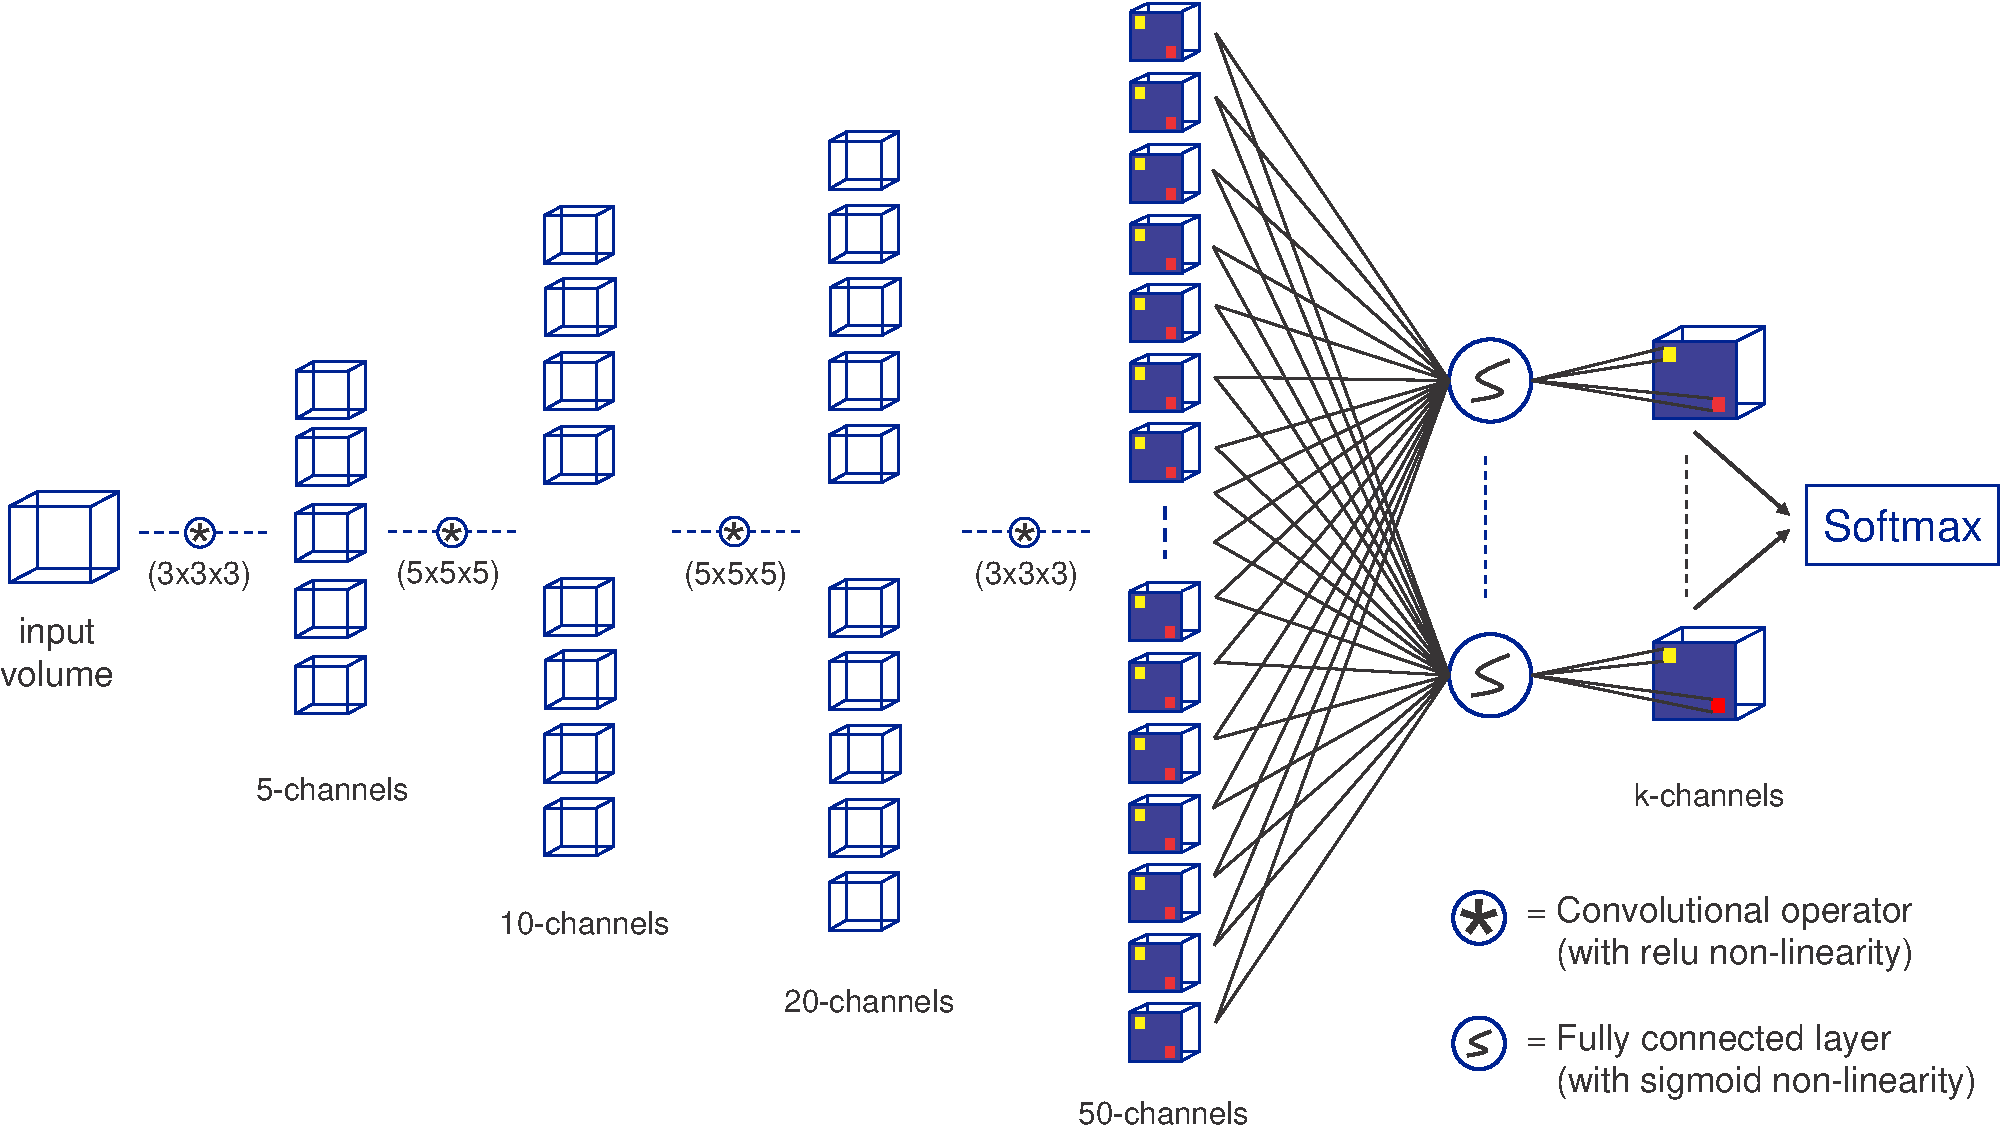
\includegraphics[width=\textwidth]{figures/model_dvn}
		\caption[Kiến trúc mô hình DeepVesselNet.]{Kiến trúc mô hình DeepVesselNet \sourcefig{\cite{tetteh2018deepvesselnet}}.}
		\label{fig:kien_truc_mang_deepvesselnet}
	\end{figure}
	Nhận thấy rằng, việc sử dụng các lớp thu giảm kích thước dữ liệu trong quá trình trích xuất đặc trưng (ví dụ lớp pooling\index{Max-pooling}) sẽ làm mất đi thông tin của đối tượng được quan tâm (thông thường chiếm lượng nhỏ thông tin), bài báo đề xuất một kiến trúc mạng gọi là \textit{Fully Convolutional Network} hay còn gọi là DeepVesselNet bao gồm bốn lớp convolution\index{Convolution} nối tiếp nhau để trích xuất thông tin, tiếp đến là một lớp convolution $1\times1\times1$ với hàm kích hoạt sigmoid\index{Sigmoid} để tổng hợp các feature map\index{Feature map} về số lớp cần phân loại, cuối cùng sử dụng lớp softmax\index{Softmax} để đưa ra kết quả phân đoạn. Kiến trúc mạng được mô tả trong \autoref{fig:kien_truc_mang_deepvesselnet}.
	
\subsection{Hàm lỗi giải quyết mất cân bằng lớp}
\label{subsec:ham_loi_giai_quyet_mat_can_bang_lop}
	Một trong những hàm lỗi thường được sử dụng trong các bài toán phân loại là cross entropy được trình bày trong \autoref{eqn:crossentropy_chuan}. Trong đó, $y$ là nhãn của điểm ảnh, $X$ là tập dữ liệu đầu vào, $\mathbf{W}$ là tập tham số của mạng, $Y_+$ và $Y_-$ lần lượt là tập điểm ảnh foreground\index{Foreground} và tập điểm ảnh background\index{Background}\footnote{Background và foreground là từ dùng để chỉ vùng nền và vùng được chú ý trong ảnh. Trong đề tài này, foregroud là hình ảnh của hệ thống mạch máu và background là các phần còn lại.}. 
	\begin{equation}
		\label{eqn:crossentropy_chuan}
		\mathcal{L} = -\frac{1}{N}\left(\sum_{y\in Y_+}\log P(y = 1|X; \mathbf{W}) + \sum_{y\in Y_-} \log P(y = 0|X; \mathbf{W})\right)
	\end{equation}
	Đối với bài toán phân tích hình ảnh y khoa, đối tượng được quan tâm (mạch máu, đường biên tế bào,\ldots) thường chiếm ít số lượng điểm ảnh. Do đó, sử dụng hàm lỗi cross entropy chuẩn có thể dẫn tới quá trình huấn luyện thiên vị về phát hiện background hơn là phát hiện đối tượng được quan tâm. Để khắc phục vấn đề này, Xie và Tu \cite{xie2015holistically} đã đề xuất hàm lỗi 
	\begin{equation}
		\label{eqn:crossentropy_can_bang_lop}
		\mathcal{L}(\mathbf{W}) = -\beta\sum_{j\in Y_+}\log P(y_j = 1|X; \mathbf{W}) - (1 - \beta) \sum_{j\in Y_-}\log P(y_j = 0|X; \mathbf{W})
	\end{equation}
	để giải quyết mất cân bằng lớp. Trong đó, $y_j$ là nhãn của điểm ảnh thứ $j$, $Y_+$ và $Y_-$ là tập điểm ảnh foreground và tập điểm ảnh background, $\beta$ và $1 - \beta$ là trọng số lớp với $\beta = \frac{|Y_-|}{|Y|}$ và $1 - \beta = \frac{|Y_+|}{|Y|}$, $X$ là tập dữ liệu đầu vào, $\mathbf{W}$ là tập tham số của mạng. $P(.)$ là xác suất từ lớp cuối của mạng. Khi mất cân bằng lớp với số lượng các điểm ảnh background nhiều hơn số lượng các điểm ảnh foreground thì $|Y_-| > |Y_+|$, do vậy, $\beta > 1 - \beta$. Khi đó, ảnh hưởng của các điểm ảnh foreground sẽ tăng lên, ảnh hưởng của các điểm ảnh background sẽ giảm đi. Điều này giúp cân bằng lại đóng góp của background và foreground tới giá trị lỗi. Tuy nhiên, hàm lỗi này lại tạo ra hai thách thức khác.
	
	Thứ nhất, \textit{sự không ổn định về số.} Việc tính toán gradient\index{Gradient}\footnote{Gradient của một hàm $f(x_1, x_2, ..., x_n)$ được ký hiệu $\triangledown f$ là một vec-tơ $n$ chiều, mà mỗi thành phần trong vec-tơ đó là một đạo hàm riêng phần (partial derivative) theo từng biến của hàm $f$.}không ổn định về số đối với những tập huấn luyện lớn do giá trị lỗi lớn. Trong \autoref{eqn:crossentropy_chuan}, hệ số $\frac{1}{N}$ giúp điều chỉnh giá trị lỗi cuối cùng về giá trị lỗi trung bình. Hệ số này đảm bảo rằng gradient ổn định và không phụ thuộc vào kích thước tập huấn luyện $N$. Tuy nhiên, \autoref{eqn:crossentropy_can_bang_lop} không đảm bảo được điều này. Ví dụ, cho một dữ liệu cân bằng, ta có $\beta = 1 - \beta = 0.5$. Khi tăng kích thước của tập dữ liệu thì $\beta$ và $1 - \beta$ không thay đổi. Số lượng phần tử tăng lên khiến cho giá trị lỗi tăng lên, từ đó tạo ra sự không ổn định của hàm lỗi.
\newpage
	Thứ hai, \textit{tỉ lệ false positive\footnote{False positive là trường hợp dự đoán sai cho điểm ảnh background.}cao.} Đối tượng được quan tâm trong hình ảnh y khoa thường chỉ chiếm ít hơn 5\% số điểm ảnh. Khi đó $1 - \beta < 0.05$, điều này làm cho việc đoán sai 95 điểm ảnh background sẽ đóng góp vào giá trị lỗi ít hơn đóng góp của việc dự đoán sai 5 điểm ảnh foreground, tức là hình phạt cho dự đoán sai trên background ít hơn hình phạt cho dự đoán sai trên foreground. Điều này dẫn tới dự đoán sai trên background nhiều đồng nghĩa tỉ lệ false positive cao. Do đó, giá trị recall cao trong khi giá trị precision thấp.
	
	Để khắc phục những thách thức này, bài báo đề xuất một cách tính trọng số khác cho các lớp đối tượng và tăng thêm mức phạt cho trường hợp false positive. Công thức hàm lỗi này được trình bày như sau.
	\begin{align}
		\mathcal{L}(\mathbf{W}) &= \mathcal{L}_1(\mathbf{W}) + \mathcal{L}_2(\mathbf{W}) \label{eqn:crossentropy_fpcorrection} \\ 
		\mathcal{L}_1(\mathbf{W}) &= -\frac{1}{|Y_+|}\sum_{j\in Y_+}\log P(y_j = 1|X; \mathbf{W}) - \frac{1}{|Y_-|}\sum_{j\in Y_-}\log P(y_j = 0|X; \mathbf{W}) \nonumber \\
		\mathcal{L}_2(\mathbf{W}) &= -\frac{\gamma_1}{|Y_+|}\sum_{j\in Y_{f+}}\log P(y_j = 0|X; \mathbf{W}) - \frac{\gamma_2}{|Y_-|}\sum_{j\in Y_{f-}}\log P(y_j = 1|X; \mathbf{W}) \nonumber \\
		\gamma_1 &= 0.5 + \frac{1}{|Y_{f+}|}\sum_{j\in Y_{f+}}|P(y_j = 0|X; \mathbf{W}) - 0.5| \nonumber \\
		\gamma_2 &= 0.5 + \frac{1}{|Y_{f-}|}\sum_{j\in Y_{f-}}|P(y_j = 1|X; \mathbf{W}) - 0.5|, \nonumber
	\end{align}
	trong đó, $\mathcal{L}_1$ là phiên bản ổn định hơn về số của \autoref{eqn:crossentropy_can_bang_lop}. Nó vừa giải quyết được vấn đề mất cân bằng lớp, vừa điều chỉnh giá trị lỗi về giá trị trung bình mặc cho kích thước của tập dữ liệu thay đổi nhờ có các hệ số $\frac{1}{|Y_+|}$, $\frac{1}{|Y_-|}$. $\mathcal{L}_2$ được đưa ra để tăng thêm mức phạt cho trường hợp dự đoán sai. Tuy nhiên, do không mong muốn tỉ lệ mức phạt cho false positive ($Y_{f+}$) và false negative ($Y_{f-}$) bằng nhau, bài báo đưa ra hệ số $\gamma_1$ và $\gamma_2$ để tăng thêm mức phạt cho các trường hợp dự đoán sai. Trong đó, trọng số cho trường hợp false positive cao hơn trọng số cho trường hợp false negative.
